\documentclass{article}
\usepackage{polski}
\usepackage[utf8]{inputenc}
\usepackage{float}
\usepackage{graphicx}
\usepackage{caption}
\usepackage{subcaption}
\usepackage{ragged2e}
\usepackage{blindtext}
\usepackage{hyperref}
\usepackage{amsmath}
\usepackage{amssymb}
\graphicspath{ {../plots/} }
\begin{document}
\author{Jakub Ogrodowczyk}
\AddToHook{cmd/section/before}{\clearpage}

\section{Clique}
\begin{figure}[htp]
    \centering
      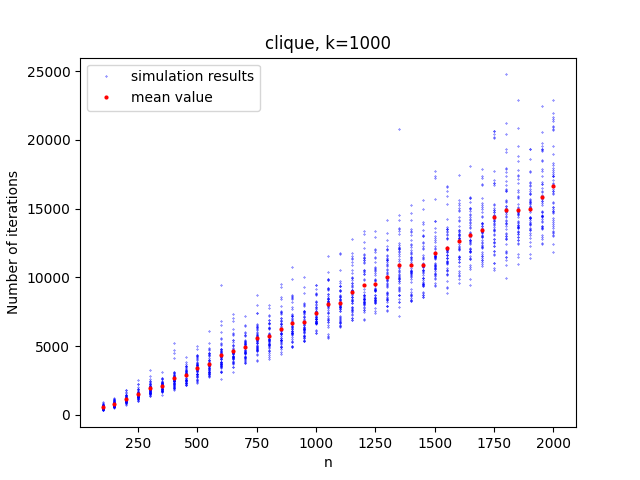
\includegraphics[width=0.5\linewidth]{clique.png}
      \label{fig:clique}
\end{figure}
\begin{figure}[H]
  \centering
  \begin{subfigure}{.475\textwidth}
    \centering
    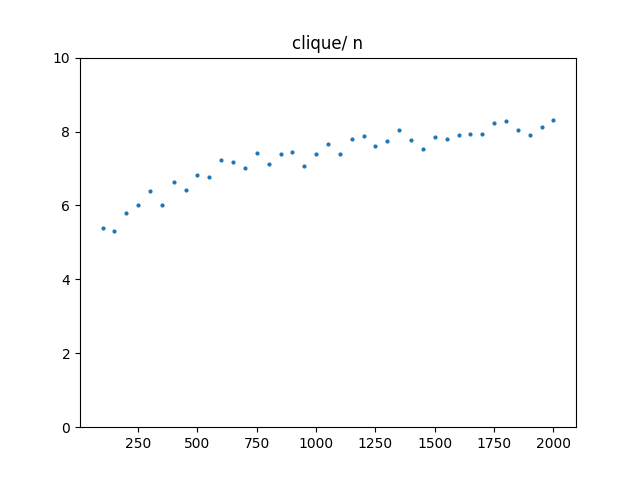
\includegraphics[width=\textwidth]{clique_n.png}
    \caption{\( \frac{\text{clique}(n)}{n} \)}
    \label{fig:clique_n}
  \end{subfigure}%
  \begin{subfigure}{.475\textwidth}
    \centering
    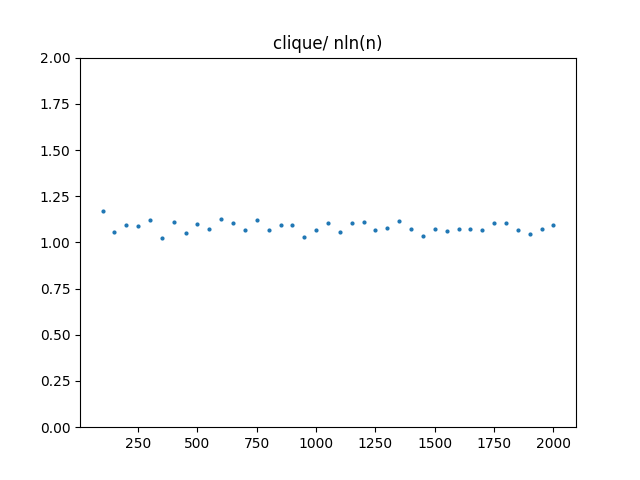
\includegraphics[width=\textwidth]{clique_nlnn.png}
    \caption{\( \frac{\text{clique}(n)}{nln(n)} \)}
    \label{fig:clique_nlnn}
  \end{subfigure}%
  \hfill
  \begin{subfigure}{.475\textwidth}
    \centering
    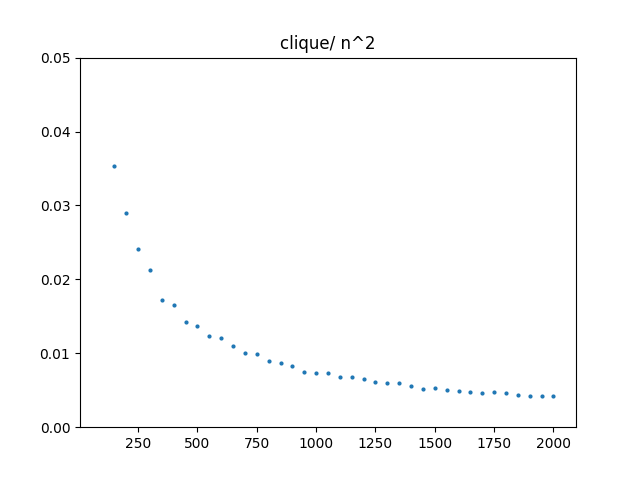
\includegraphics[width=\textwidth]{clique_nn.png}
    \caption{\( \frac{\text{clique}(n)}{n^2} \)}
    \label{fig:clique_nn}
  \end{subfigure}%
  \begin{subfigure}{.475\textwidth}
    \centering
    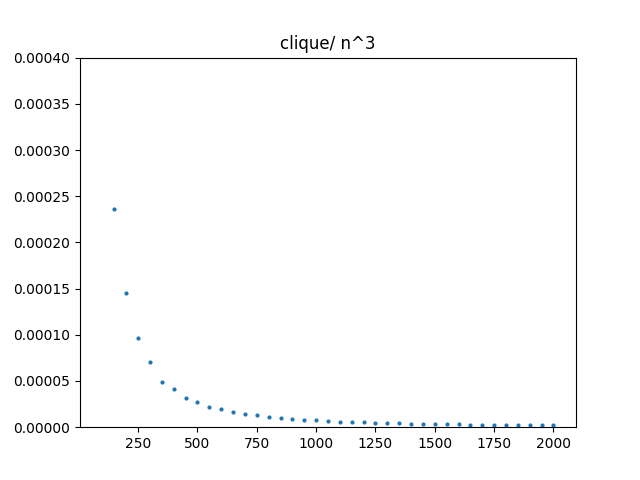
\includegraphics[width=\textwidth]{clique_nnn.png}
    \caption{\( \frac{\text{clique}(n)}{n^3} \)}
    \label{fig:clique_nnn}
  \end{subfigure}%
  \caption{Wykresy pomagające wyznaczyć asymptotykę funkcji.}
\end{figure}
\center{Hipoteza:}
\[\text{Clique}(n)=O(nln(n))\]

\section{Path}
\begin{figure}[htp]
    \centering
      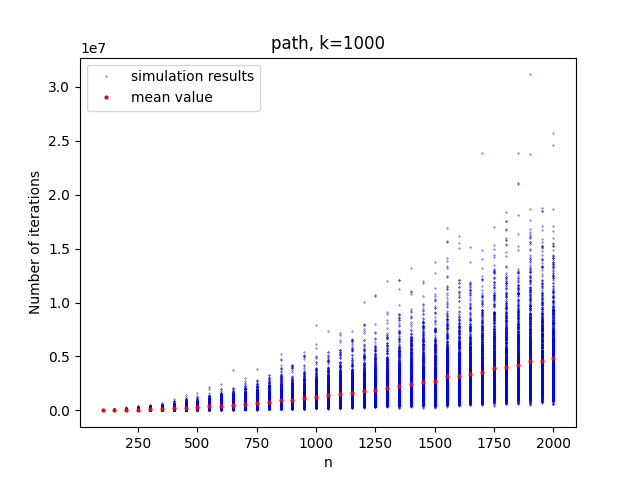
\includegraphics[width=0.5\linewidth]{path.png}
      \label{fig:path}
\end{figure}
\begin{figure}[H]
  \centering
  \begin{subfigure}{.475\textwidth}
    \centering
    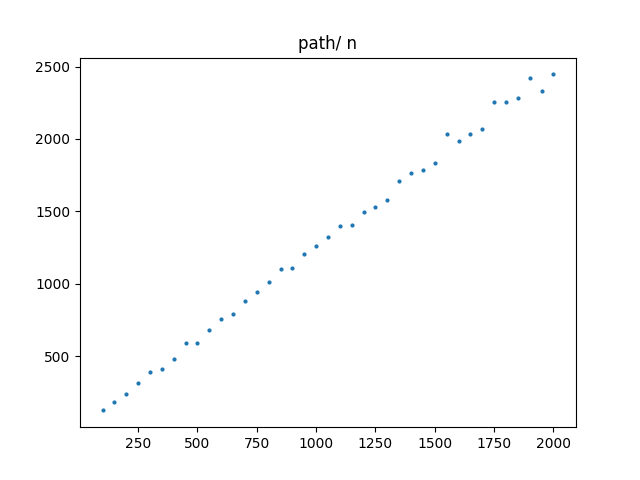
\includegraphics[width=\textwidth]{path_n.png}
    \caption{\( \frac{\text{path}(n)}{n} \)}
    \label{fig:path_n}
  \end{subfigure}%
  \begin{subfigure}{.475\textwidth}
    \centering
    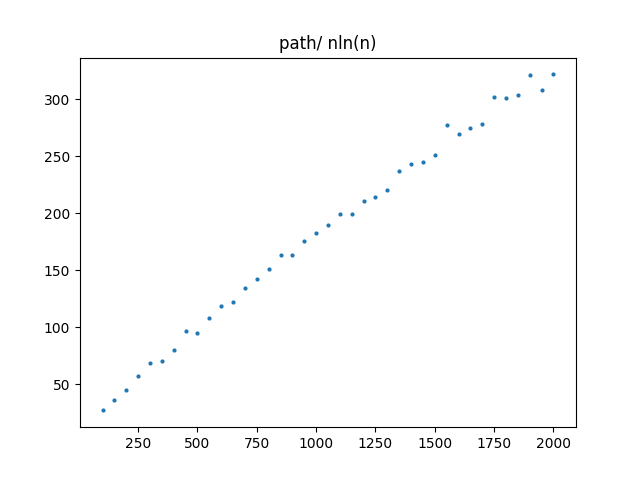
\includegraphics[width=\textwidth]{path_nlnn.png}
    \caption{\( \frac{\text{path}(n)}{nln(n)} \)}
    \label{fig:path_nlnn}
  \end{subfigure}%
  \hfill
  \begin{subfigure}{.475\textwidth}
    \centering
    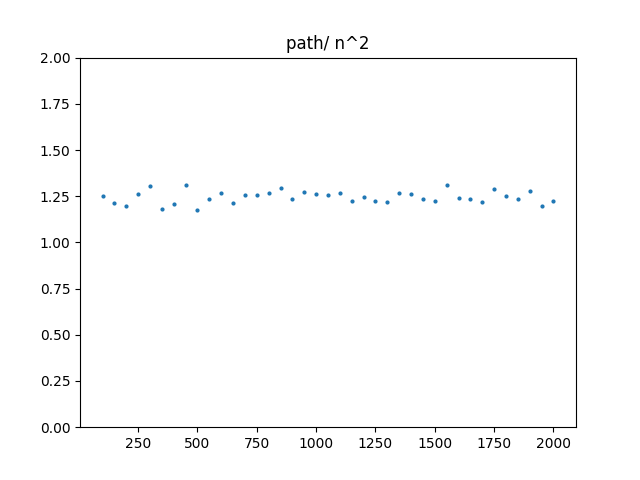
\includegraphics[width=\textwidth]{path_nn.png}
    \caption{\( \frac{\text{path}(n)}{n^2} \)}
    \label{fig:path_nn}
  \end{subfigure}%
  \begin{subfigure}{.475\textwidth}
    \centering
    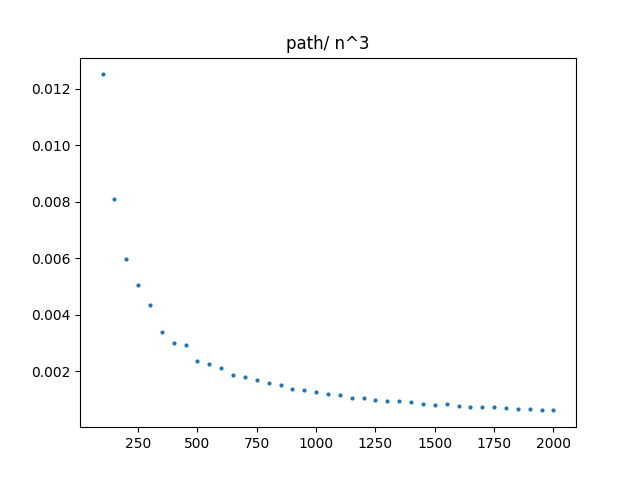
\includegraphics[width=\textwidth]{path_nnn.png}
    \caption{\( \frac{\text{path}(n)}{n^3} \)}
    \label{fig:path_nnn}
  \end{subfigure}%
  \caption{Wykresy pomagające wyznaczyć asymptotykę funkcji.}
\end{figure}
\center{Hipoteza:}
\[\text{path}(n)=O(n^2)\]

\section{Path, start in the beginning node}
\begin{figure}[htp]
  \centering
    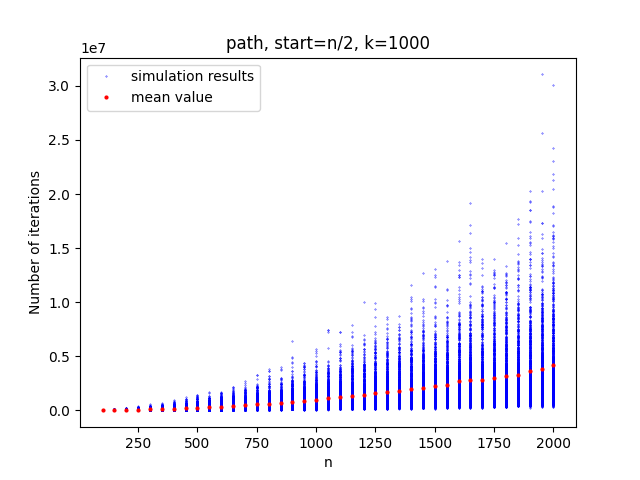
\includegraphics[width=0.5\linewidth]{path_beginning.png}
    \label{fig:path_beginning}
\end{figure}
\begin{figure}[H]
  \centering
  \begin{subfigure}{.475\textwidth}
    \centering
    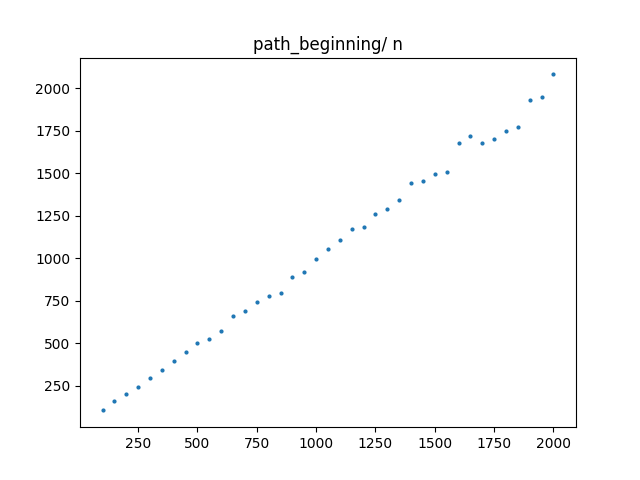
\includegraphics[width=\textwidth]{path_beginning_n.png}
    \caption{\( \frac{\text{path}_0(n)}{n} \)}
    \label{fig:path_beginning_n}
  \end{subfigure}%
  \begin{subfigure}{.475\textwidth}
    \centering
    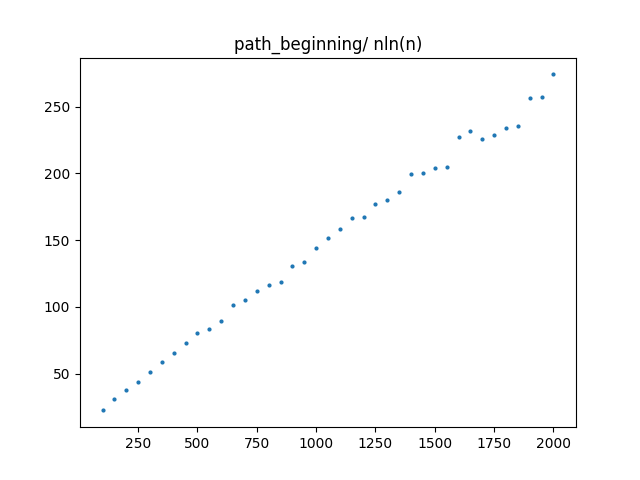
\includegraphics[width=\textwidth]{path_beginning_nlnn.png}
    \caption{\( \frac{\text{path}_0(n)}{nln(n)} \)}
    \label{fig:path_beginning_nlnn}
  \end{subfigure}%
  \hfill
  \begin{subfigure}{.475\textwidth}
    \centering
    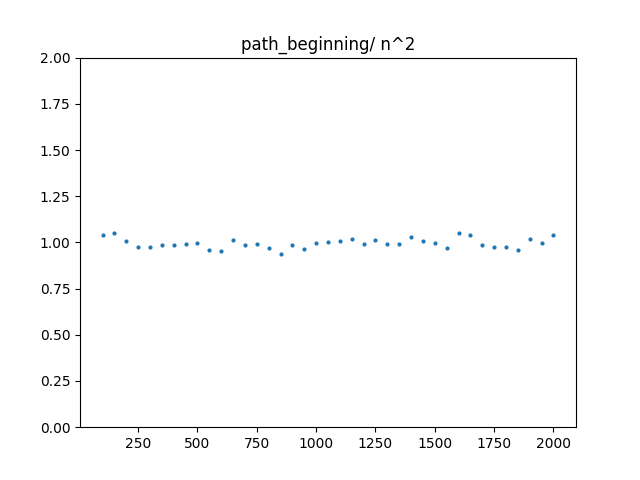
\includegraphics[width=\textwidth]{path_beginning_nn.png}
    \caption{\( \frac{\text{path}_0(n)}{n^2} \)}
    \label{fig:path_beginning_nn}
  \end{subfigure}%
  \begin{subfigure}{.475\textwidth}
    \centering
    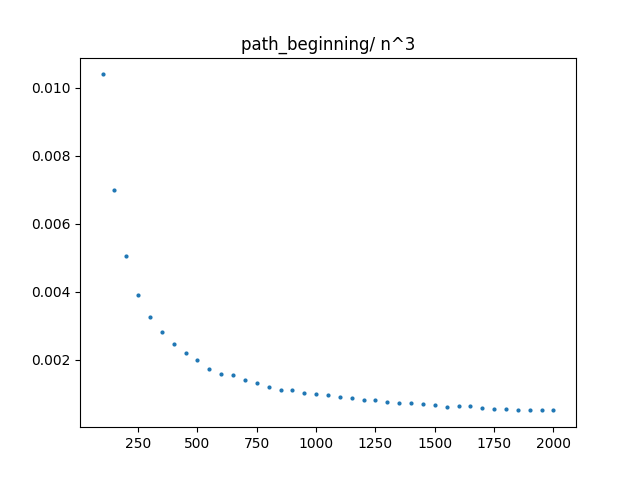
\includegraphics[width=\textwidth]{path_beginning_nnn.png}
    \caption{\( \frac{\text{path}_0(n)}{n^3} \)}
    \label{fig:path_beginning_nnn}
  \end{subfigure}%
  \caption{Wykresy pomagające wyznaczyć asymptotykę funkcji.}
\end{figure}
\center{Hipoteza:}
\[\text{path}_0(n)=O(n^2)\]

\section{Binary Tree}
\begin{figure}[htp]
  \centering
    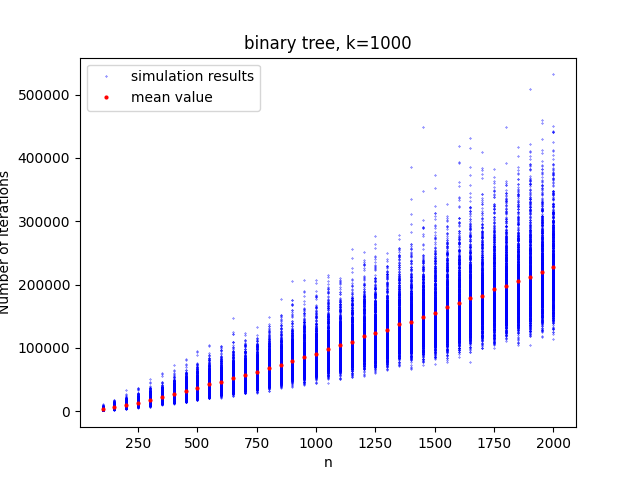
\includegraphics[width=0.5\linewidth]{binary_tree.png}
    \label{fig:binary_tree}
\end{figure}
\begin{figure}[H]
  \centering
  \begin{subfigure}{.475\textwidth}
    \centering
    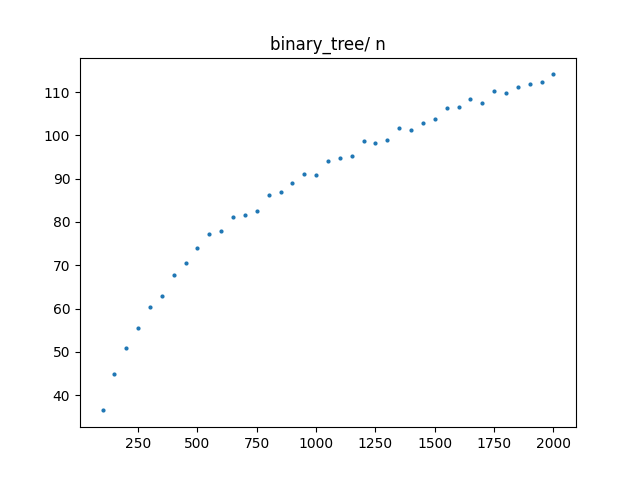
\includegraphics[width=\textwidth]{binary_tree_n.png}
    \caption{\( \frac{\text{binarytree}(n)}{n} \)}
    \label{fig:binary_tree_n}
  \end{subfigure}%
  \begin{subfigure}{.475\textwidth}
    \centering
    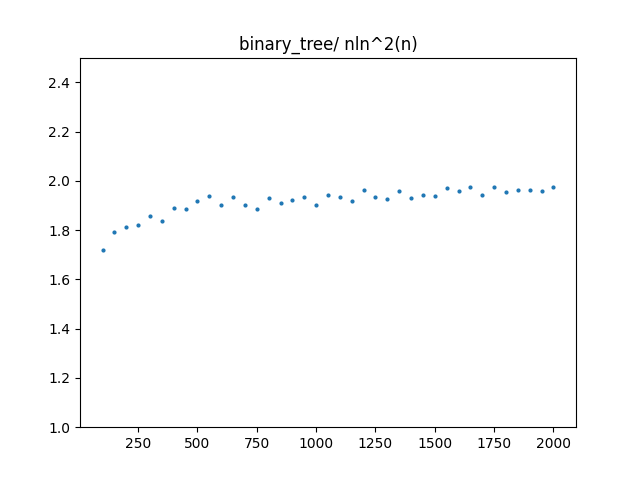
\includegraphics[width=\textwidth]{binary_tree_nlnnlnn.png}
    \caption{\( \frac{\text{binarytree}(n)}{nln^2(n)} \)}
    \label{fig:binary_tree_nlnn}
  \end{subfigure}%
  \hfill
  \begin{subfigure}{.475\textwidth}
    \centering
    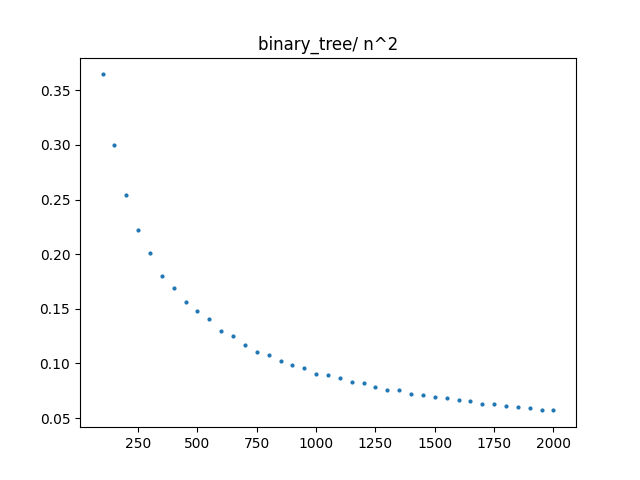
\includegraphics[width=\textwidth]{binary_tree_nn.png}
    \caption{\( \frac{\text{binarytree}(n)}{n^2} \)}
    \label{fig:binary_tree_nn}
  \end{subfigure}%
  \begin{subfigure}{.475\textwidth}
    \centering
    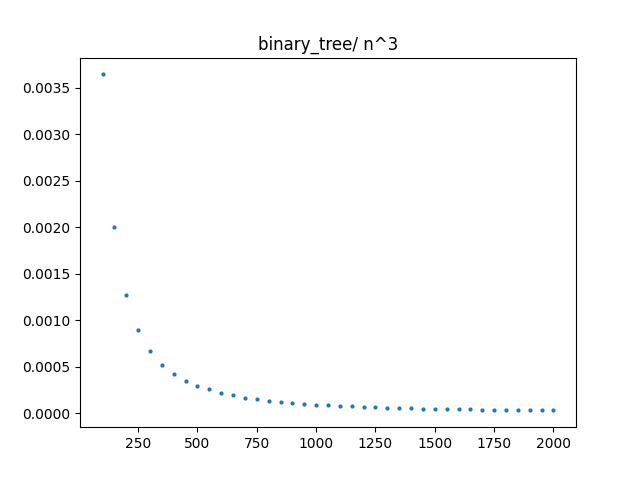
\includegraphics[width=\textwidth]{binary_tree_nnn.png}
    \caption{\( \frac{\text{binarytree}(n)}{n^3} \)}
    \label{fig:binary_tree_nnn}
  \end{subfigure}%
  \caption{Wykresy pomagające wyznaczyć asymptotykę funkcji.}
  \label{fig:bn}
\end{figure}
\center{Hipoteza:}
\[\text{binarytree}(n)=O(nln^2(n))\]

\section{Lollipop}
\begin{figure}[htp]
  \centering
    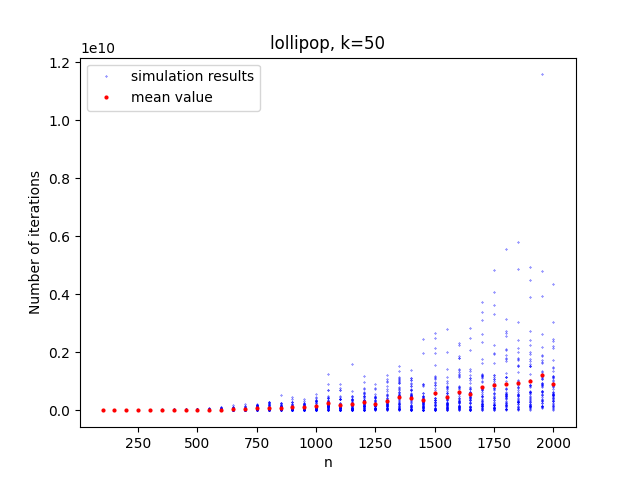
\includegraphics[width=0.5\linewidth]{lollipop.png}
    \label{fig:lollipop}
\end{figure}
\begin{figure}[H]
  \centering
  \begin{subfigure}{.475\textwidth}
    \centering
    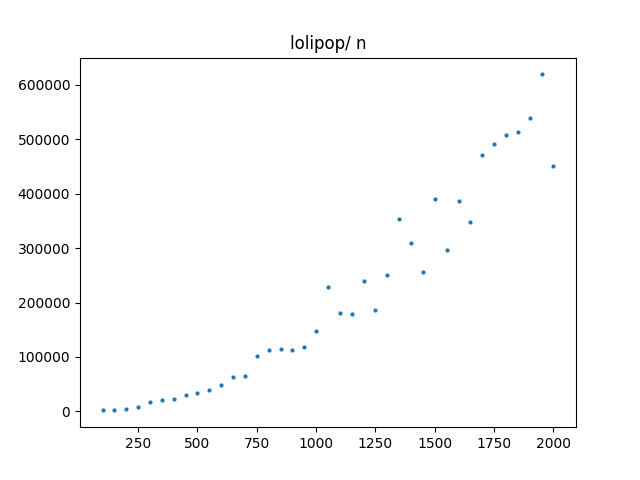
\includegraphics[width=\textwidth]{lollipop_n.png}
    \caption{\( \frac{\text{lollipop}(n)}{n} \)}
    \label{fig:lollipop_n}
  \end{subfigure}%
  \begin{subfigure}{.475\textwidth}
    \centering
    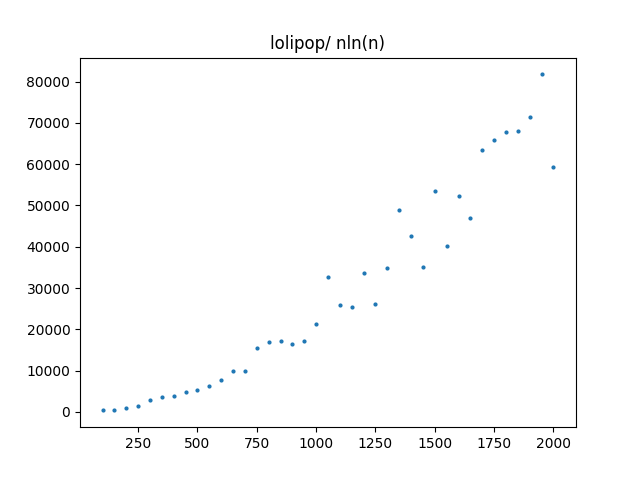
\includegraphics[width=\textwidth]{lollipop_nlnn.png}
    \caption{\( \frac{\text{lollipop}(n)}{nln(n)} \)}
    \label{fig:lollipop_nlnn}
  \end{subfigure}%
  \hfill
  \begin{subfigure}{.475\textwidth}
    \centering
    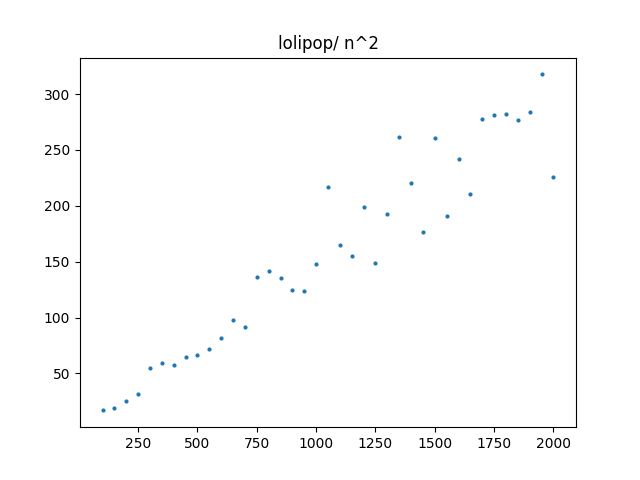
\includegraphics[width=\textwidth]{lollipop_nn.png}
    \caption{\( \frac{\text{lollipop}(n)}{n^2} \)}
    \label{fig:lollipop_nn}
  \end{subfigure}%
  \begin{subfigure}{.475\textwidth}
    \centering
    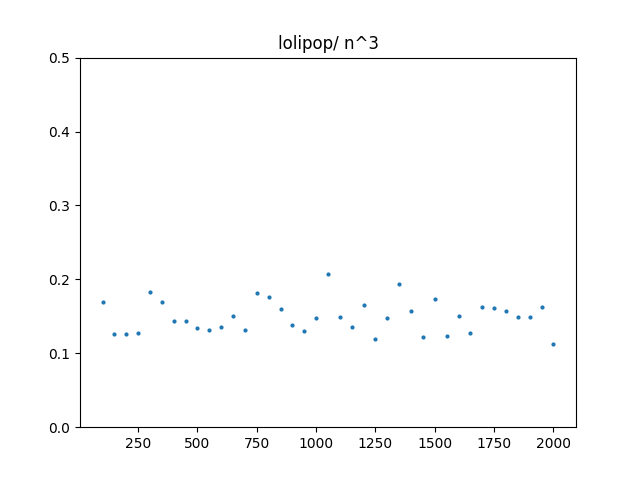
\includegraphics[width=\textwidth]{lollipop_nnn.png}
    \caption{\( \frac{\text{lollipop}(n)}{n^3} \)}
    \label{fig:lollipop_nnn}
  \end{subfigure}%
  \caption{Wykresy pomagające wyznaczyć asymptotykę funkcji.}
  \label{fig:bn}
\end{figure}
\center{Hipoteza:}
\[\text{lollipop}(n)=O(n^3)\]

\justifying
\section{Wnioski}
Z ciekawych rzeczy, zauważyć możemy, że przy symulacji ścieżki, niezależnie
od miejsca startu (początek / środek) mamy i tak tę samą złożoność. Poza tym
możemy zaobserwować bardzo dużą wariancję, przykładowo w jednej symulacji lollipopa
przy \(n = 1950\) wykonane zostało aż \(11,578,127,039\) iteracji, podczas gdy
średnia wynosiła około 200 mln.
\subsection*{symulacja}
Jeśli chodzi o rzeczy ściśle powiązane z częścią programistyczną tego zadania, to
przeprowadziłem eksperyment porównujący wydajność symulacji przy korzystaniu z listy
sąsiedztwa w grafie, a funkcją losową, która zwraca następny wierzchołek do odwiedzenia
(bez tworzenia żadnych struktur w pamięci, poza tablicą odwiedzonych wierzchołków).
Okazuje się, że drugie rozwiązanie jest znacznie wydajniejsze w grafach, w których
listy sąsiedztwa są na tyle długie, że nie mieszczą się w pamięci cache. Tutaj były
to klika oraz lizak. Dla kliki wydajność wzrosła około ośmiokrotnie, a dla lizaka
dwukrotnie. Dla reszty grafów, gdzie każdy wierzchołek ma niewielu sąsiądów,
wydajniejsze było stworzenie grafu i losowanie wierzchołka z listy sąsiedztwa.
\end{document}
